\documentclass[a4paper]{report}
\usepackage{RJournal}
\usepackage{moreverb}
\usepackage{booktabs}

\begin{document}

\fancyhf{}
\fancyhead[L]{\textsc{Instructions for Authors}}
\fancyhead[R]{\thepage}

\begin{article}
\title{Instructions for Authors}

\author{by The R Journal Editors}

\maketitle

\abstract{
\emph{The R Journal} is compiled using \LaTeX{} and authors are required
to submit their articles as \LaTeX{} documents. Here we provide authors
with information for preparing submissions to the \emph{Journal}.
}

\section{Introduction}

\emph{The R Journal} is the refereed journal of the R Project for Statistical
Computing \citep{ihaka:1996}.
It features short to medium length articles covering topics
that might be of interest to users or developers of R.

\emph{The R Journal} intends to reach a wide audience and have a 
thorough review process. Papers are expected to be reasonably short,
clearly written, not too technical, and of course focused on R. Authors 
of refereed articles should take care to:

\begin{itemize}
\item put their contribution in context, in particular discuss related R
  functions or packages; 
\item explain the motivation for their contribution;
\item provide code examples that are reproducible.
\end{itemize}

Following revision of the content description of The R Journal, 
from January 2017 submitted articles may include:

\begin{itemize}

\item \emph{Reviews and proposals}: surveying and discussing challenges and opportunities of potential importance for the broader R community, including proposals and proof-of-concept implementations.

\item \emph{Comparisons and benchmarking}: of implementations in base-R and contributed packages with each other, and where relevant with implementations in other software systems.

\item \emph{Applications}: demonstrating how new or existing techniques can be applied in an area of current interest using R, providing a fresh view of such analyses in R that is of benefit beyond the specific application.

\item \emph{Add-on packages}: short introductions to contributed R packages that are already available on CRAN or Bioconductor, and going beyond package vignettes in aiming to provide broader context and to attract a wider readership than package users. Authors need to make a strong case for such introductions, based for example on novelty in implementation and use of R, or the introduction of new data structures representing general architectures that invite re-use. Authors of narrower package-introduction articles may wish to consider alternatives such as The Journal of Open Source Software (\url{http://joss.theoj.org/}) or in the life sciences, the F1000 Bioconductor (\url{https://f1000research.com/channels/bioconductor}) or Rpackage (\url{https://f1000research.com/channels/rpackage}) channels.

\end{itemize}

\noindent
\emph{The R Journal} also has a \emph{News and Notes} section,
including information on:

\begin{description}

\item[Changes in R:] New features of the latest release.

\item[Changes on CRAN:] New add-on packages, manuals, binary distributions,
mirrors, etc.

\item[News from the Bioconductor project:] Latest developments from 
\url{www.bioconductor.org}.

\item[R Foundation News:] Donations to and new members of The R Foundation.

\item[Conferences:] Upcoming R-related conferences and reports from
conferences.

\end{description}

The purpose of this document is to describe to all prospective authors how
to prepare a submission for \emph{The R Journal}.

\section{Preparing a submission}

The following files provide a template for preparing an article for submission
to \emph{The R Journal}:

\begin{description}

\item[\LaTeX{} style file:] \file{RJournal.sty}.

\item[Master \LaTeX{} file:] \file{RJwrapper.tex}. This includes the file
  \file{RJtemplate.tex}, which is not itself a complete \LaTeX{} document
  (it has no \verb|\begin{document}| or \verb|\end{document}|).

\item[Article template:] \file{RJtemplate.tex}.

\item[Bibliography template:] \file{RJreferences.bib}.

\end{description}

The steps involved in preparing an article for submission to \emph{The
  R Journal} are as follows:

\begin{itemize}

\item Download \file{RJwrapper.tex}, \file{RJtemplate.tex},
and \file{RJournal.sty}.

\item Rename \file{RJtemplate.tex} using the authors' last names in lower case 
separated by hyphens, (e.g.\ \file{smith-jones.tex}). Replace its
contents with the contents of your article.

\item Create a \file{Yourlastname.bib} BibTeX file and add
\verb|\bibliography{Yourlastname}| at the end of \file{Yourlastname.tex}.

\item Modify \file{RJwrapper.tex} to include \file{yourname.tex} rather
than \file{RJtemplate.tex}. Include any strictly essential \LaTeX{} 
\verb|\usepackage| commands in the modified \file{RJwrapper.tex}.

\item Run \code{tools::texi2pdf} on \file{RJwrapper.tex} to produce 
\file{RJwrapper.pdf}, using \code{clean=FALSE} to help in debugging 
if necessary.

\item Iterate until \file{RJwrapper.pdf} looks right.

\item Then submit the following files to the Editor-in-Chief:
  \begin{itemize}
  \item The modified \file{RJwrapper.tex}
  \item \file{RJwrapper.pdf}
  \item \file{yourname.tex}
  \item \file{yourname.bib}
  \item all necessary figure files (only PDF or PNG files are accepted)
  \item an R script permitting the reproduction of examples in your submission and small data files --- use built-in data sets where sensible, see below. 
  \item Do not include \file{RJournal.sty} or style files for other latex packages needed by your article.
  \end{itemize}
\end{itemize}

\section{Reproducible research}

The results presented in figures and tables should be reproducible:
either the R code to generate the result should be included in a code
listing in the article, or a separate script file that generates the
results should be submitted with the article. Articles that include
extensive code listings should also provide a script file to help
reviewers step through the code without retyping it.

\section{Language}

Articles in \emph{The R Journal} are written in English. We accept
consistent British and American spelling along with other national
variations. We encourage authors for whom English is not their first
language to have their papers edited by a competent copy-editor. We
encourage all authors to conform to accepted norms of grammar and style,
and to avoid sexist language, such as the use of `he' for individuals
of indefinite gender.

\section{Copyright}

Starting from 2017, all published articles are licensed under the Creative Commons Attribution 4.0 International license (CC BY 4.0, \url{http://creativecommons.org/licenses/by/4.0}. Until the end of 2016, and including issue 2016-2, published articles were licensed under the Creative Commons Attribution 3.0 Unported license (CC BY 3.0, \url{http://creativecommons.org/licenses/by/3.0/}).

\section{References and attribution}

The R Journal follows customary academic practice in requiring that text in submissions and code and text in software be properly attributed. Quoted text must be attributed correctly and included in references; plagiarism and self-plagiarism will lead to rejection of submissions.

\section{Marking text}

The \LaTeX{} style file \file{RJournal.sty} provides some useful commands for marking up words and phrases related to softare (as inspired by Texinfo). Please use these commands and the other mark-up facilities described in this section rather than attempting to format output and other elements visually. Unless it is absolutely necessary, please refrain from introducing additional idiosyncratic mark-up---for example, for programming languages.

The commands provided are:

\begin{description}

\item[\code{$\backslash$ \\code\{\var{sample-code}\}}]
indicates text that is a literal example of a piece of a program.
For example, \verb|\code{rows <- nrow(X)}| is typeset as
\code{rows <- nrow(X)}. The \verb|\code| command should also
be used for keyboard input and the names of objects, functions and
arguments. Class names should be quoted; for example \verb|\code{"lm"}| is
typeset as \code{"lm"}. This is a regular command so special latex characters like \verb|_| and \verb|\| will need to be escaped.

\item[\code{$\backslash$ \\samp\{\var{text}\}}]
indicates text that is a literal example of a sequence of
characters. It should be used whenever parts of inline code
could be confused with text, for example \verb|\samp{R CMD check}| is
typeset as \samp{R CMD check} and  e.g. \verb|\samp{...}| would give
\samp{...}. 

\item[\code{$\backslash$ \\file\{\var{file-name}\}}]
indicates the name of a file. For example,
\verb|\file{RJwrapper.tex}| is typeset as \file{RJwrapper.tex}.

\item[\code{$\backslash$ \\dfn\{\var{term}\}}]
indicates the introductory or defining use of a term.
For example, \verb|\dfn{environment}| is typeset as
\dfn{environment}.

\end{description}

We also provide the following markup:

\begin{description}
\item[\code{$\backslash$ \\strong}]
emphasizes text more strongly than  \verb|\emph|.
For example, \verb|\strong{Note:}| is typeset as \strong{Note:}.

\item[\code{$\backslash$ \\pkg}]
indicates an R package. For example,
\verb|\pkg{MASS}| is typeset as \pkg{MASS}.

\item[\code{$\backslash$ \\CRANpkg}]
indicates an R package on CRAN, and includes a hyper-link to the
corresponding web page. For example,
\verb|\CRANpkg{Rcpp}| is typeset as \CRANpkg{Rcpp}.

\item[\code{$\backslash$ \\BIOpkg}]
indicates a Bioconductor package, and includes a hyper-link to
the corresponding page on the Bioconductor web site. For example,
\verb|\BIOpkg{affy}| is typeset as \BIOpkg{affy}.

\item[\code{$\backslash$ \\url}] indicates a URL.
For example,\\ \verb|\url{http://cran.r-project.org/}| is typeset
as \url{http://cran.r-project.org/}.

\end{description}

Note that no markup is necessary to typeset R. Likewise, no markup
should be used to typeset the names of external software. In particular,
the \verb|\pkg| command is reserved for R packages.

\subsection{Examples}

Include examples with the verbatim-like \verb|example| environment. The text is printed in a fixed-width font, and indented but not filled.

If you want to intermingle code and latex, you can use the \verb|example*| environment, which is a wrapper for \verb|altt|.

\begin{example}
# This is some example code. Please make sure to wrap lines to around 80
# characters so that they fit nicely within the body of the text.
#
# Use indentation and spacing to improve the readability of code
# listings where possible, e.g. put spaces after commas and around
# equals signs.
# 
# For example, don't do:
f <- function(y, debug=FALSE) {
stopifnot(is.numeric(y) && length(y) == 1)
if (y<0 && debug)
message("Y is negative")
invisible(y)
}

# Instead do:
f <- function(y, debug = FALSE) {
  stopifnot(is.numeric(y) && length(y) == 1)
  if (y < 0 && debug) {
    message("Y is negative")
  }
  invisible(y)
}
\end{example}

\subsection{Sectioning, titles, and abstract}

Use only \verb|\section| and \verb|\subsection| commands, not
\verb|\section*| or \verb|\subsection*|.

The title of the article should be set with initial capitals, as in
\texttt{\\title\{Drawing Diagrams with R\}}. Only the initial word of
section and subsection titles should be capitalized; for example,
\verb|\section{Starting at the end}|. 

If the title includes a package name, the name should be formatted
with the \verb|\pkg| command. This ensures that the package name is
correctly typeset when it appears in the Table of Contents of \emph{The R
Journal}. Note that \verb|\pkg| is the only markup that should be used
inside a title.

Every article should include an abstract of no more than 150 words. The abstract
is entered with the \verb|\abstract| command, and should appear immediately
after \verb|\maketitle| at the beginning of the article. The abstract
should not contain any citations or references.

\subsection{Author information}

Authors' names only should be given at the beginning of the article,
following the title, using the \verb|\author| command. The list of
authors should begin with the word ``by''. All other information is
given in the `signature block' at the end of the article (see
immediately below). For example,
\verb|\author{by Ross Ihaka and Robert Gentleman}|.

The article should end with a signature block giving contact information
for each author. For example

\begin{verbatim}
\address{Paul Murrell\\
  Department of Statistics\\
  The University of Auckland\\
  New Zealand\\
  \email{paul@stat.auckland.ac.nz}}
\end{verbatim}  

\subsection{Mathematics}

\emph{The R Journal} does not prescribe specific \LaTeX{} mark-up for mathematics: Use
mark-up that is conventional in your field. We do, however, encourage authors to
follow sound \LaTeX{} practices. 

\begin{itemize}

\item For example, use proper mathematical operators: 
Do not write \verb|log(x)|, which will be typeset as $log(x)$, but rather \verb|\log(x)|,
which will appear as $\log(x)$. 

\item Similarly, use \verb|\left| and \verb|\right| with
delimiters in mathematical expressions in preference to bare delimiters:
Do not write
\begin{verbatim}
\sum_{i=1}^{n}(X_{i}^{\prime} - 
  \overline{X}^{\prime})^2
\end{verbatim}
which will be typeset as $\sum_{1=1}^{n}(X_{i}^{\prime} - \overline{X}^{\prime})^2$,
but rather
\begin{verbatim}
\sum_{i=1}^{n}\left(X_{i}^{\prime} - 
  \overline{X}^{\prime}\right)^2
\end{verbatim}
which will appear as $\sum_{i=1}^{n}\left(X_{i}^{\prime} - \overline{X}^{\prime}\right)^2$.

Try to stick to symbols from amssymb and avoid alternative symbol fonts.

\end{itemize}


\section{Figures and tables}

Horizontal lines in tables should use commands from the
booktabs package, i.e.\ \verb|\toprule| for the top of the table,
\verb|\bottomrule| for the bottom of the table, and \verb|\midrule|
for any horizontal lines within the table (see Table \ref{table:onecoltab}).

\begin{table}
\centering
\begin{tabular}{lcc}
\toprule
   & Left & Right \\
\midrule
Up & 1  &  2 \\
Down &  3 & 4 \\
\bottomrule
\end{tabular}
\caption{\label{table:onecoltab}
A simple table with booktabs formatting.}
\end{table}

Figures should be submitted as PDF or PNG format files; other formats are not accepted.

Variants of the figure and table environments that span the full width of the document are avialable: these are called \verb|widefigure| and \verb|widetable|.  Figures~\ref{fig:regular} and \ref{fig:wide} show the difference between the regular and wide figure variants.

\begin{figure}[htbp]
  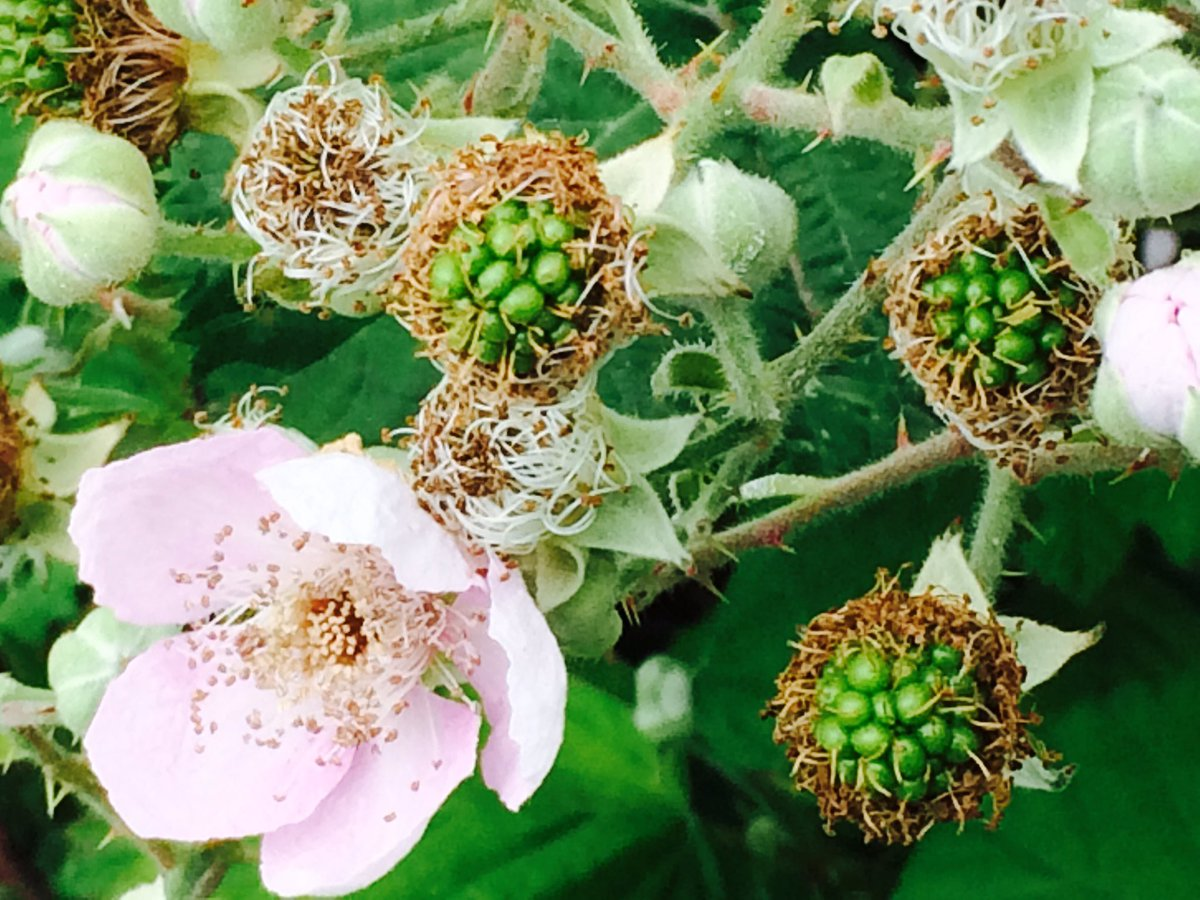
\includegraphics[width=0.5\linewidth]{tests/wild_blackberries.png}%
  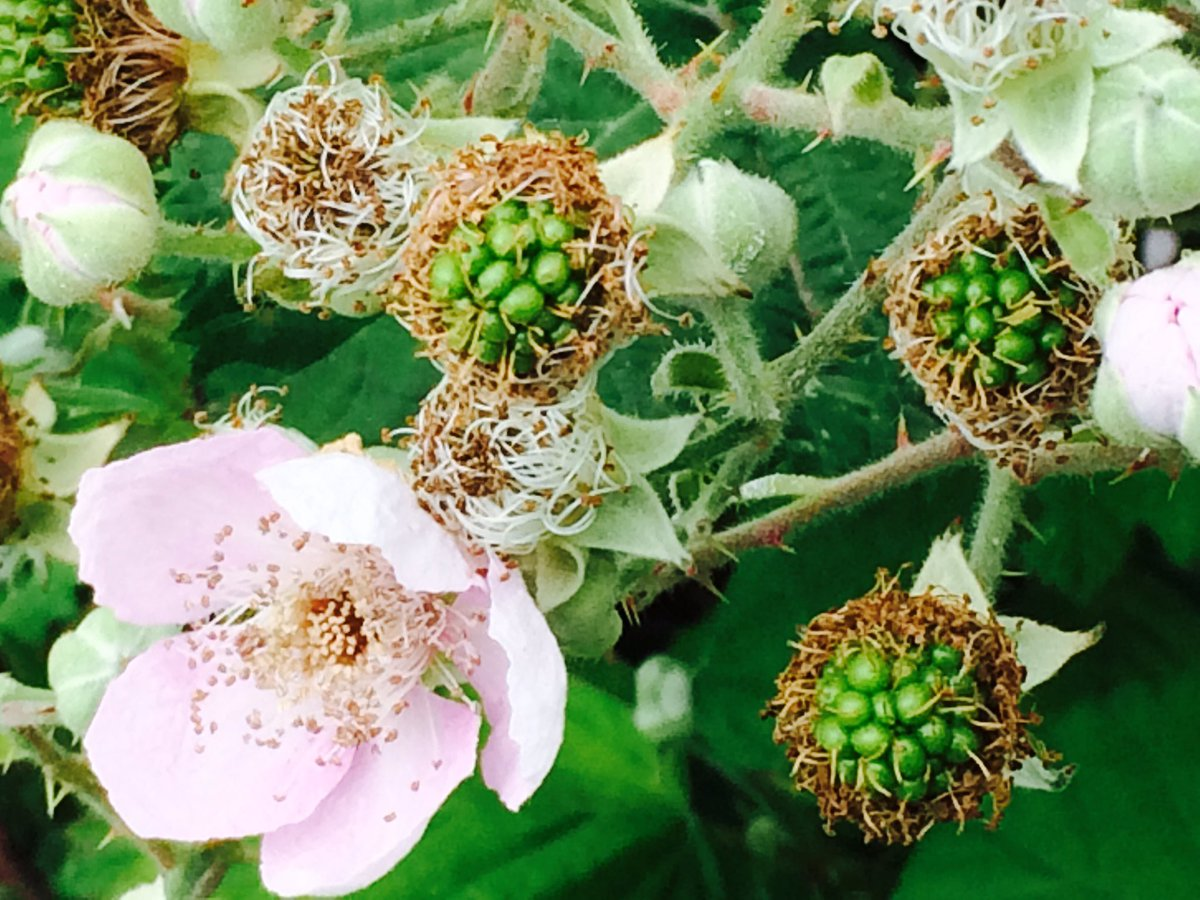
\includegraphics[width=0.5\linewidth]{tests/wild_blackberries.png}
  \caption{This figure should be the same width as the text.}
  \label{fig:regular}
\end{figure}

\begin{widefigure}[htbp]
  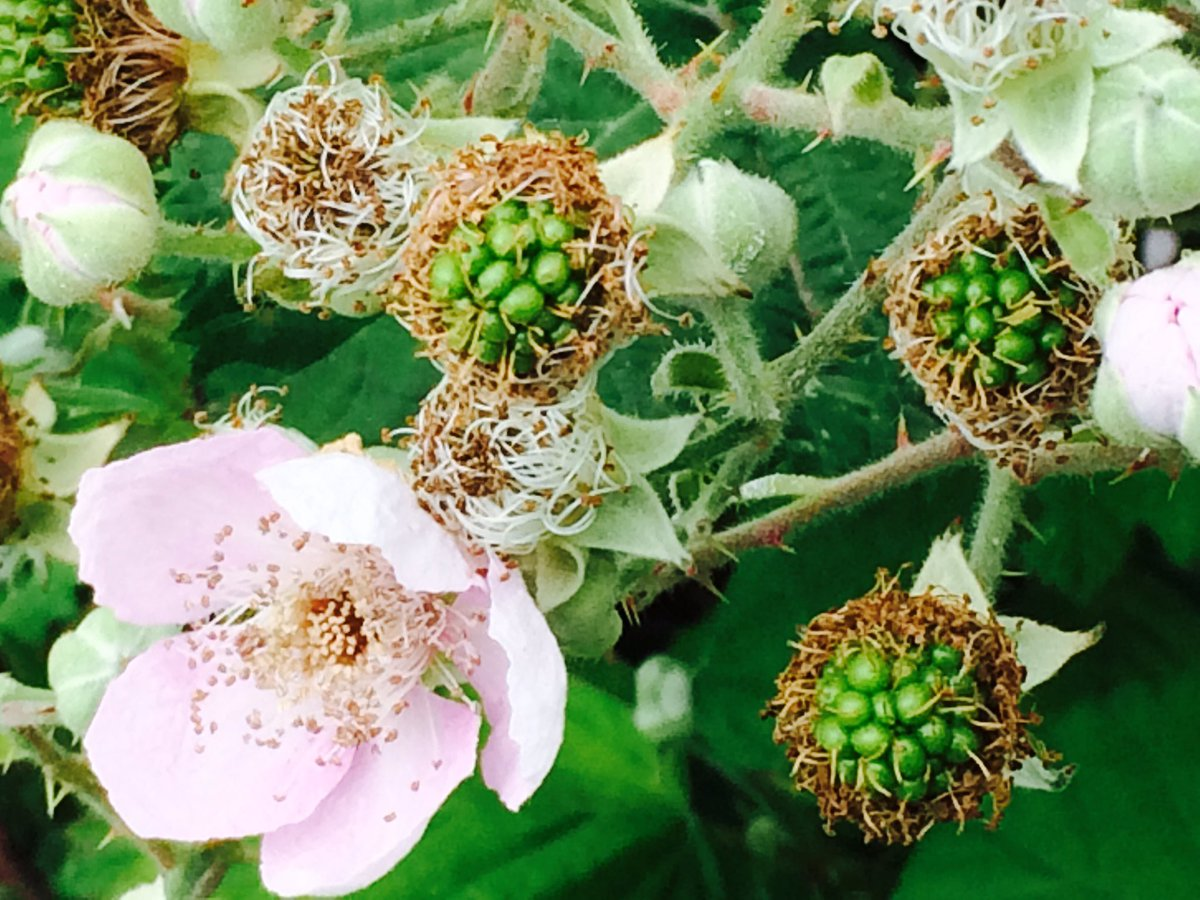
\includegraphics[width=0.5\linewidth]{tests/wild_blackberries.png}%
  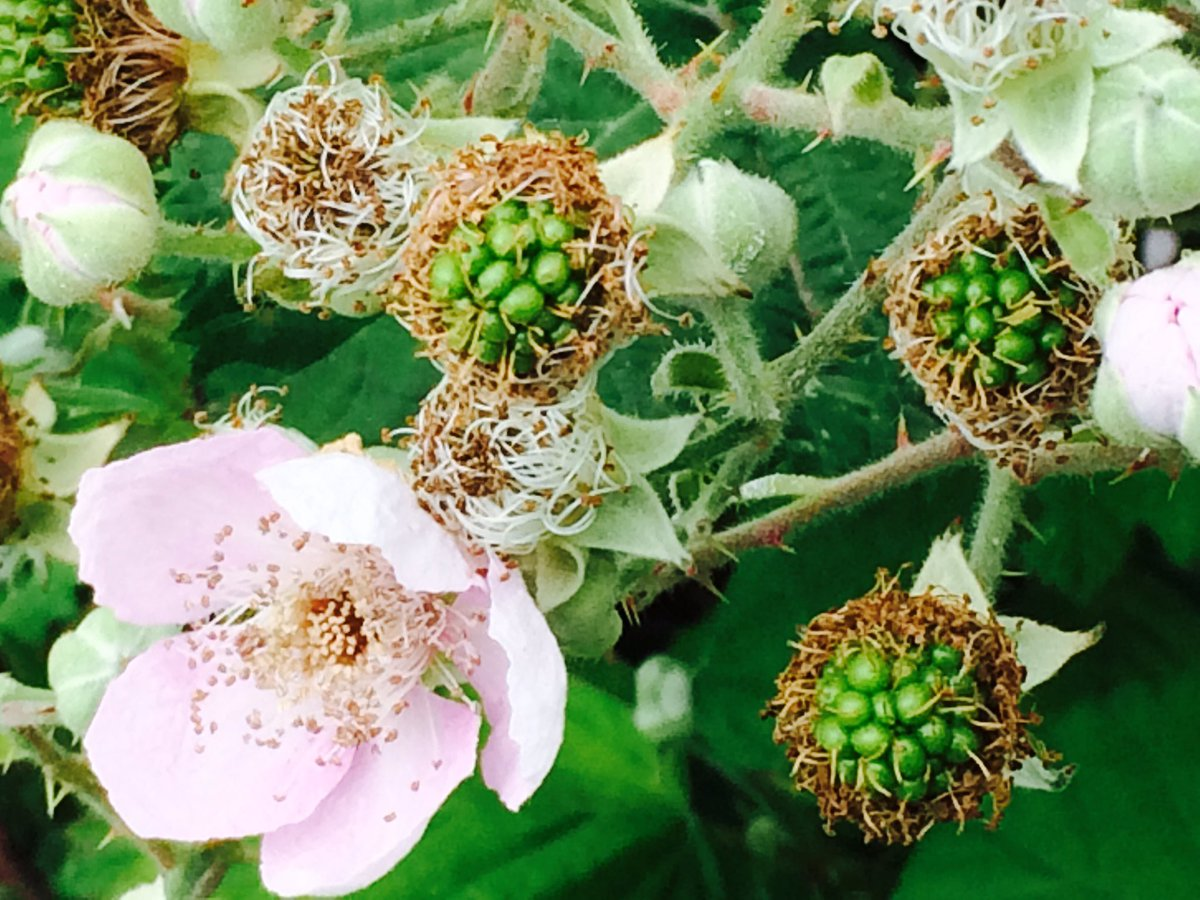
\includegraphics[width=0.5\linewidth]{tests/wild_blackberries.png}
  \caption{This figure should span the page, but the caption should be the same width as the text. Use this environment sparingly}
  \label{fig:wide}
\end{widefigure}

For structuring a figure into subfigures, use the subcaption package.

\section{References}
\label{sec:references}

The standard way to produce citations for \emph{The R Journal} is via the natbib
\verb|\citep| and \verb|\citet| commands (and their relatives)
and a \file{.bib} file that contains the
references in {\sc Bib}\TeX{} format\footnote{We use the \pkg{natbib}
package for citations.}. The citation in the first
paragraph of this style guide is of the form
\verb|\citep{ihaka:1996}|. Figure \ref{figure:bibexample}
shows an example file called \file{example.bib} which contains
a single reference. Note that inclusion of the DOI () bibtex field is desirable whenever a referenced item has a DOI; if \verb|doi| is used, \verb|url| should in general not be used.

A bibliography is produced from \file{example.bib}
by placing the following line in \file{yourfilename.tex}:
\begin{verbatim}
\bibliography{yourfilename}
\end{verbatim}
and running \code{pdflatex} then \code{bibtex} on the file
\file{yourfilename.tex}, then running \code{pdflatex} as many times as
necessary until \LaTeX{} stops complaining about undefined citations.  In R, you can use \code{tools::texi2pdf()} to automate this process, as this is what is used in production.

It is not necessary to include the \code{natbib} package or a bibliography style: these are included in the RJournal style file.

\begin{figure}[htbp]
\centering
\begin{boxedverbatim}
@ARTICLE{R:Ihaka+Gentleman:1996,
  AUTHOR = {Ross Ihaka and Robert Gentleman},
  TITLE = {R: A Language for Data Analysis and Graphics},
  JOURNAL = {Journal of Computational and Graphical Statistics},
  YEAR = 1996,
  VOLUME = 5,
  NUMBER = 3,
  PAGES = {299--314},
  DOI = {10.1080/10618600.1996.10474713}
}
\end{boxedverbatim}
\caption{The contents of a file called \file{example.bib}.}
\label{figure:bibexample}
\end{figure}

BibTeX will ignore capitalization in titles, unless words are
protected inside curly braces, e.g.\ \verb|R| will appear as ``r'',
whereas \verb|{R}| will appear correctly as ``R''. Ensure that proper
names in titles are protected. Similarly, in the author field,
corporate authors will not appear correctly unless protected, e.g. a
bibtex entry with
\begin{verbatim}
AUTHOR = {The R Journal Editors}
\end{verbatim}
will appear in the bibliography as ``TRJ Editors'' and should be
protected with double braces:
\begin{verbatim}
AUTHOR = {{The R Journal Editors}}
\end{verbatim}
Including the DOI of the reference is very desirable and may become compulsory soon.

\subsection{Citing packages}

The first time a package is cited in the text, excluding the abstract,
it should be followed by a formal citation, such as the one generated
by the \verb|citation()| function in R. The first citation of a CRAN
package should use \verb|\CRANpkg| and the first citation of a Bioconductor
package should use \verb|\BIOpkg|. Further citations use \verb|\pkg|
and need not be followed by a citation.

The BibTeX entry for an R package should not use the \verb|\pkg|
command to format the package name in the \code{TITLE} field.

\subsection{Citing R}

Articles in \emph{The R Journal} do not include a citation of R itself.

\section{Acknowledgment}

Parts of this style guide were adapted from documentation originally
prepared by Kurt Hornik and Friedrich Leisch for the \emph{R Journal}
\LaTeX{} style file.

\section{Changelog}

\begin{itemize}
  \item v0.5, 2008/09/04 --- Copy and edit Rnews.dtx.
  
\item v0.6, 2009/05/05 --- Require \pkg{tikz} for decoration of contents page.
  Require \pkg{amsmath}, \pkg{pslatex}, \pkg{palatino}, \pkg{mathpazo}. Define
  hyperref colors. (Re)define \verb|\sectionhead|, \verb|\abstract|. Simplify equation
  numbering. Restyled colophon. Defined \verb|Sin|, \verb|Sout| and \verb|Schunk| enrionments.
  \verb|\acronym| non longer changes text.
  
\item v0.7, 2010/07/01 -- Used \verb|\phantomsection| in chapter head so that
  hyperlinks in toc jump to place above not below article title. Added \verb|\review|
  command to set up head for book reviews - treated as hybrid of chapter and
  section. Removed markup for mathematics as not recommended for use. Changed
  Rnews references to RJournal references. Removed \verb|\startRnews| as unused.
  
\item v0.8, 2010/12/29 --- Added |table| environment for one-column tables.

\item v0.9, 2012/01/13 --- Disabled ligatures in \verb|\code|.

\item v0.10, 2013/01/08 --- Added back-links from bibliography

\item v0.11, 2013/01/11 --- Dropped two-column format. Dropped custom figure and
  table environments.  Use placeins package to keep figures and tables (now
  floating) under control.

\item v0.12, 2013/04/11 --- Tweaks to one column format. Use inconsolata
  for code. Switch example to verbatim; add example* for alltt. Slightly
  increased spacing between lines and paragraphs. Don't use alternating 
  headers. Support for wide figures (widefigure) and tables (widetable)

\item v0.13 2013/08/27 --- Added \verb|\BIOpkg| for Bioconductor packages.

\item v0.14 2017/01/09 --- Revised Introduction to adapt classes of solicited submissions to changing needs and high submission volumes of single package articles. Added hooks for licence and plagiarism.

\end{itemize}

\end{article}

\bibliography{RJreferences}

\end{document}
